\documentclass[14pt,ignorenonframetext,aspectratio = 1610]{beamer}
\setbeamertemplate{caption}[numbered]
\setbeamertemplate{caption label separator}{: }
\setbeamercolor{caption name}{fg=normal text.fg}
\beamertemplatenavigationsymbolsempty
\usepackage{lmodern}
\usepackage{amssymb,amsmath}
\usepackage{ifxetex,ifluatex}
\usepackage{fixltx2e} % provides \textsubscript
\ifnum 0\ifxetex 1\fi\ifluatex 1\fi=0 % if pdftex
  \usepackage[T1]{fontenc}
  \usepackage[utf8]{inputenc}
\else % if luatex or xelatex
  \ifxetex
    \usepackage{mathspec}
  \else
    \usepackage{fontspec}
  \fi
  \defaultfontfeatures{Ligatures=TeX,Scale=MatchLowercase}
    \setmainfont[]{Georgia}
    \setmonofont[Mapping=tex-ansi]{Lucida Console}
\fi
\usefonttheme{serif} % use mainfont rather than sansfont for slide text
% use upquote if available, for straight quotes in verbatim environments
\IfFileExists{upquote.sty}{\usepackage{upquote}}{}
% use microtype if available
\IfFileExists{microtype.sty}{%
\usepackage{microtype}
\UseMicrotypeSet[protrusion]{basicmath} % disable protrusion for tt fonts
}{}
\newif\ifbibliography
\hypersetup{
            pdftitle={Acute effects of ambient exposures},
            pdfauthor={Brooke Anderson},
            pdfborder={0 0 0},
            breaklinks=true}
%\urlstyle{same}  % Use monospace font for urls
\usepackage{color}
\usepackage{fancyvrb}
\newcommand{\VerbBar}{|}
\newcommand{\VERB}{\Verb[commandchars=\\\{\}]}
\DefineVerbatimEnvironment{Highlighting}{Verbatim}{commandchars=\\\{\}}
% Add ',fontsize=\small' for more characters per line
\usepackage{framed}
\definecolor{shadecolor}{RGB}{248,248,248}
\newenvironment{Shaded}{\begin{snugshade}}{\end{snugshade}}
\newcommand{\KeywordTok}[1]{\textcolor[rgb]{0.13,0.29,0.53}{\textbf{#1}}}
\newcommand{\DataTypeTok}[1]{\textcolor[rgb]{0.13,0.29,0.53}{#1}}
\newcommand{\DecValTok}[1]{\textcolor[rgb]{0.00,0.00,0.81}{#1}}
\newcommand{\BaseNTok}[1]{\textcolor[rgb]{0.00,0.00,0.81}{#1}}
\newcommand{\FloatTok}[1]{\textcolor[rgb]{0.00,0.00,0.81}{#1}}
\newcommand{\ConstantTok}[1]{\textcolor[rgb]{0.00,0.00,0.00}{#1}}
\newcommand{\CharTok}[1]{\textcolor[rgb]{0.31,0.60,0.02}{#1}}
\newcommand{\SpecialCharTok}[1]{\textcolor[rgb]{0.00,0.00,0.00}{#1}}
\newcommand{\StringTok}[1]{\textcolor[rgb]{0.31,0.60,0.02}{#1}}
\newcommand{\VerbatimStringTok}[1]{\textcolor[rgb]{0.31,0.60,0.02}{#1}}
\newcommand{\SpecialStringTok}[1]{\textcolor[rgb]{0.31,0.60,0.02}{#1}}
\newcommand{\ImportTok}[1]{#1}
\newcommand{\CommentTok}[1]{\textcolor[rgb]{0.56,0.35,0.01}{\textit{#1}}}
\newcommand{\DocumentationTok}[1]{\textcolor[rgb]{0.56,0.35,0.01}{\textbf{\textit{#1}}}}
\newcommand{\AnnotationTok}[1]{\textcolor[rgb]{0.56,0.35,0.01}{\textbf{\textit{#1}}}}
\newcommand{\CommentVarTok}[1]{\textcolor[rgb]{0.56,0.35,0.01}{\textbf{\textit{#1}}}}
\newcommand{\OtherTok}[1]{\textcolor[rgb]{0.56,0.35,0.01}{#1}}
\newcommand{\FunctionTok}[1]{\textcolor[rgb]{0.00,0.00,0.00}{#1}}
\newcommand{\VariableTok}[1]{\textcolor[rgb]{0.00,0.00,0.00}{#1}}
\newcommand{\ControlFlowTok}[1]{\textcolor[rgb]{0.13,0.29,0.53}{\textbf{#1}}}
\newcommand{\OperatorTok}[1]{\textcolor[rgb]{0.81,0.36,0.00}{\textbf{#1}}}
\newcommand{\BuiltInTok}[1]{#1}
\newcommand{\ExtensionTok}[1]{#1}
\newcommand{\PreprocessorTok}[1]{\textcolor[rgb]{0.56,0.35,0.01}{\textit{#1}}}
\newcommand{\AttributeTok}[1]{\textcolor[rgb]{0.77,0.63,0.00}{#1}}
\newcommand{\RegionMarkerTok}[1]{#1}
\newcommand{\InformationTok}[1]{\textcolor[rgb]{0.56,0.35,0.01}{\textbf{\textit{#1}}}}
\newcommand{\WarningTok}[1]{\textcolor[rgb]{0.56,0.35,0.01}{\textbf{\textit{#1}}}}
\newcommand{\AlertTok}[1]{\textcolor[rgb]{0.94,0.16,0.16}{#1}}
\newcommand{\ErrorTok}[1]{\textcolor[rgb]{0.64,0.00,0.00}{\textbf{#1}}}
\newcommand{\NormalTok}[1]{#1}
\usepackage{graphicx,grffile}
\makeatletter
\def\maxwidth{\ifdim\Gin@nat@width>\linewidth\linewidth\else\Gin@nat@width\fi}
\def\maxheight{\ifdim\Gin@nat@height>\textheight0.8\textheight\else\Gin@nat@height\fi}
\makeatother
% Scale images if necessary, so that they will not overflow the page
% margins by default, and it is still possible to overwrite the defaults
% using explicit options in \includegraphics[width, height, ...]{}
\setkeys{Gin}{width=\maxwidth,height=\maxheight,keepaspectratio}

% Prevent slide breaks in the middle of a paragraph:
\widowpenalties 1 10000
\raggedbottom

\AtBeginPart{
  \let\insertpartnumber\relax
  \let\partname\relax
  \frame{\partpage}
}
\AtBeginSection{
  \ifbibliography
  \else
    \let\insertsectionnumber\relax
    \let\sectionname\relax
    \frame{\sectionpage}
  \fi
}
\AtBeginSubsection{
  \let\insertsubsectionnumber\relax
  \let\subsectionname\relax
  \frame{\subsectionpage}
}

\setlength{\parindent}{0pt}
\setlength{\parskip}{6pt plus 2pt minus 1pt}
\setlength{\emergencystretch}{3em}  % prevent overfull lines
\providecommand{\tightlist}{%
  \setlength{\itemsep}{0pt}\setlength{\parskip}{0pt}}
\setcounter{secnumdepth}{0}


\title[Short Title]{Acute effects of ambient exposures}
\subtitle{Time series and case-crossover studies}
\author[
Anderson
]{Brooke Anderson}
\institute[
CSU
]{
ERHS \\
Colorado State University
}
\date[
02/12/18
]{
February 12, 2018
}

% ------------------------------------------------------------------------------------------------
% BELOW ARE MY ADDITIONS
% ------------------------------------------------------------------------------------------------

% ------------------------------------------------------------------------------------------------
%	PACKAGE LIST
% ------------------------------------------------------------------------------------------------
\usepackage{
booktabs,
%fontspec,
graphicx,
multicol,
pgfplots,
ragged2e,
tabularx,
tikz,
wasysym,
hyperref,
hanging,
multirow,
eso-pic,
}

\usepackage[export]{adjustbox}
% ------------------------------------------------------------------------------------------------
%	GRAPHICS PATH
% ------------------------------------------------------------------------------------------------
\graphicspath{{./figs/}}


% ------------------------------------------------------------------------------------------------
%	TABLE OF CONTENTS
% ------------------------------------------------------------------------------------------------
\useoutertheme[subsection=false,shadow]{miniframes}
\setbeamertemplate{section in toc}[sections numbered]
\setbeamertemplate{subsection in toc}[subsections numbered]

% ------------------------------------------------------------------------------------------------
%	ITEMIZE
% ------------------------------------------------------------------------------------------------
\setbeamertemplate{itemize item}{$\bullet$}
\setbeamertemplate{itemize subitem}{$\circ$}
\setbeamertemplate{itemize subsubitem}{$\bullet$}

\setlength{\parskip}{0.5em}

% ------------------------------------------------------------------------------------------------
%	COLORS
% ------------------------------------------------------------------------------------------------

% sthlm Colors
\definecolor{sthlmLightBlue}{RGB}{90,200,250}
\definecolor{sthlmBlue}{RGB}{52,170,220}
\definecolor{sthlmDarkBlue}{RGB}{0,122,255}
\definecolor{sthlmLightRed}{RGB}{255,45,85}
\definecolor{sthlmRed}{RGB}{255,59,48}
\definecolor{sthlmLightYellow}{RGB}{255,204,0}
\definecolor{sthlmYellow}{RGB}{255,149,0}
\definecolor{sthlmPurple}{RGB}{88,86,214}
\definecolor{sthlmGreen}{RGB}{76,217,100}
\definecolor{sthlmGrey}{RGB}{142,142,147}
\definecolor{sthlmLightGrey}{RGB}{233,233,233}
\definecolor{sthlmDarkGrey}{RGB}{61,61,70}

% General
\setbeamercolor{normal text}{fg=sthlmDarkGrey}
\hypersetup{colorlinks=true, urlcolor=sthlmDarkBlue, linkcolor=sthlmDarkGrey, citecolor=sthlmDarkBlue}
\setbeamercolor{structure}{fg=sthlmDarkGrey}
\setbeamercolor{alerted text}{fg=sthlmRed}
\setbeamercolor{example text}{fg=white}
\setbeamercolor{copyright text}{fg=sthlmLightBlue}
\setbeamercolor{palette primary}{fg=sthlmDarkGrey}
\setbeamercolor{palette secondary}{fg=sthlmDarkGrey,bg=sthlmLightGrey}
\setbeamercolor{palette tertiary}{fg=black,bg=sthlmDarkGrey}
\setbeamercolor{palette quaternary}{fg=white, bg=sthlmDarkGrey}

\setbeamercolor{mini frame}{bg=sthlmLightGrey}
\setbeamercolor{section in head/foot}{fg=sthlmDarkGrey, bg=sthlmLightGrey}

% Titlepage
\setbeamercolor{title}{parent=normal text}
\setbeamercolor{subtitle}{parent=normal text}
\setbeamercolor{institute}{parent=normal text}

% Content
\setbeamercolor{frametitle}{parent=palette quaternary}

% Blocks
\setbeamercolor{block title}{fg=white,bg=sthlmDarkBlue}
\setbeamercolor{block body}{fg=sthlmDarkGrey, bg=sthlmLightGrey}
\setbeamercolor{block title example}{fg=white, bg=sthlmGreen}
\setbeamercolor{block body example}{fg=sthlmDarkGrey, bg=sthlmLightGrey}
\setbeamercolor{block title alerted}{fg=white, bg=sthlmLightRed}
\setbeamercolor{block body alerted}{fg=sthlmDarkGrey, bg=sthlmLightGrey}

% Notes
\setbeamercolor{note page}{fg=sthlmDarkGrey,bg=sthlmLightGrey}
\setbeamercolor{note title}{fg=white, bg=sthlmDarkGrey}
\setbeamercolor{note date}{parent=note title}

% Page Number
\setbeamercolor{page number in head/foot}{fg=sthlmDarkGrey}

\setbeamercolor{qed}{fg=sthlmGrey}
\setbeamercolor{itemize item}{fg=sthlmDarkBlue}
\setbeamercolor{itemize subitem}{fg=sthlmDarkBlue}
\setbeamercolor{itemize subsubitem}{fg=sthlmDarkBlue}

% ------------------------------------------------------------------------------------------------
%	FONTS
% ------------------------------------------------------------------------------------------------

% General

%% Declare fontfamilys
%\if@doNoFlama%
%	% Sans serif math option
%	\if@doSans%
%	% Sans serif math
%		\usepackage{fontspec}%
%		\setmainfont{Arial Regular}%
%	\else%
%		% Serif math
%		\usefonttheme{professionalfonts}%
%		\usepackage[no-math]{fontspec}%
%	\fi%
%	
%	\newfontfamily\Light{Arial Regular}%
%	\newfontfamily\Book{Arial Black Regular}%
%	\newfontfamily\bfseries{Arial Bold}%
%	\setsansfont{Arial Regular}%
%\else%
%	% Sans serif math option
%	\if@doSans%
%	% Sans serif math
%		\usepackage{fontspec}%
%		\setmainfont{FlamaLight}%
%	\else%
%		% Serif math
%		\usefonttheme{professionalfonts}%
%		\usepackage[no-math]{fontspec}%
%	\fi%
%	
%	\newfontfamily\Light{FlamaLight}%
%	\newfontfamily\Book{FlamaBook}%
%	\newfontfamily\bfseries{FlamaMedium}%
%	\setsansfont{FlamaLight}%
%	%\newfontfamily\texttt{SourceCodePro-Light}
%\fi%
%
%%\renewcommand\UrlFont{\texttt}
%
%% Font sizes
%
%% Titlepage
%\setbeamerfont{title}{family=\bfseries,size=\fontsize{24}{26}}
%\setbeamerfont{subtitle}{family=\Light,size=\fontsize{14}{18}}
%\setbeamerfont{subtitle}{size=\fontsize{14}{18}}
%\setbeamerfont{date}{size=\fontsize{9}{11}}
%\setbeamerfont{author}{family=\bfseries,size=\fontsize{13}{15}}
%\setbeamerfont{institute}{size=\fontsize{09}{10}}
%
%% Section
%\setbeamerfont{section title}{size*={39pt}{24pt}, family = \bfseries, series=\bfseries}% Content
%\setbeamerfont{frametitle}{family=\bfseries,size=\large}
%\setbeamerfont{copyright text}{family=\Light,size=\tiny}
%\setbeamerfont{block title}{family=\Book,size=\large}
%\setbeamerfont{block title alerted}{family=\Book,size=\large}
%\setbeamerfont{alerted text}{family=\bfseries}
%
%%Captions
%\setbeamerfont{caption name}{family=\Book}




%% ------------------------------------------------------------------------------------------------
%%	FONT ASSIGMENTS
%% ------------------------------------------------------------------------------------------------
%% Title Page
%\newfontfamily\Light{Roboto Light}
%\setbeamerfont{title}{size=\LARGE, series=\bfseries}
%\setbeamerfont{subtitle}{family=\Light, size=\small, shape=\normalfont}
%\setbeamerfont{date}{family=\Light, size=\footnotesize}
%\setbeamerfont{author}{size=\small, series=\bfseries}
%\setbeamerfont{institute}{family=\Light, size=\scriptsize}
%
%% Section
%\setbeamerfont{section title}{size=\Huge}
%
%% Content
%\setbeamerfont{frametitle}{size=\Large, series=\bfseries}
%\setbeamerfont{copyright text}{size=\tiny}
%\setbeamerfont{block title}{size=\large, series=\bfseries}
%\setbeamerfont{block title alerted}{size=\large, series=\bfseries}
%\setbeamerfont{block title example}{size=\large, series=\bfseries}
%
%\setbeamerfont{caption}{size=\small}
%\setbeamerfont{caption name}{family=\small}

% ------------------------------------------------------------------------------------------------
%	FONT ASSIGMENTS
% ------------------------------------------------------------------------------------------------
% Title Page
%\newfontfamily\Light{Roboto Light}
\setbeamerfont{title}{size=\LARGE, series=\bfseries}
\setbeamerfont{subtitle}{size=\small, shape=\normalfont}
\setbeamerfont{date}{size=\footnotesize}
\setbeamerfont{author}{size=\small, series=\bfseries}
\setbeamerfont{institute}{size=\scriptsize}

% Section
\setbeamerfont{section title}{size=\Huge}

% Content
\setbeamerfont{frametitle}{size=\Large, series=\bfseries}
\setbeamerfont{copyright text}{size=\tiny}
\setbeamerfont{block title}{size=\large, series=\bfseries}
\setbeamerfont{block title alerted}{size=\large, series=\bfseries}
\setbeamerfont{block title example}{size=\large, series=\bfseries}

\setbeamerfont{caption}{size=\small}
\setbeamerfont{caption name}{family=\small}

% ------------------------------------------------------------------------------------------------
%	TITLE PAGE
% ------------------------------------------------------------------------------------------------

\newcommand\AtPageUpperRight[1]{\AtPageUpperLeft{%
 \put(\LenToUnit{\paperwidth},\LenToUnit{0\paperheight}){#1}%
 }}%
\newcommand\AtPageLowerRight[1]{\AtPageLowerLeft{%
 \put(\LenToUnit{\paperwidth},\LenToUnit{0\paperheight}){#1}%
 }}%

%\AddToShipoutPictureBG*{% Add picture to current page
%  \AtStockLowerLeft{% Add picture to lower-left corner of paper stock
%    \includegraphics[width=\stockwidth,height=\stockheight]{tiger}}% http://latex.tug.org/texlive/devsrc/Master/texmf-dist/doc/generic/pstricks/images/tiger.eps
%}

% Titlepage structure
\def\maketitle{\ifbeamer@inframe\titlepage\else\frame[plain]{\titlepage}\fi}
\def\titlepage{\usebeamertemplate{title page}}
\setbeamertemplate{title page}
%\frame[plain]{\titlepage}
{
	% Add background to title page
  	%\AddToShipoutPictureFG*{\includegraphics[width=\paperwidth]{backgroundiegs.pdf}}
	\AddToShipoutPictureFG*{
		\AtPageLowerRight{\put(-95, 0){
			\includegraphics[width=.2\paperwidth]{title_graphic.pdf}}}}
	%\AddToShipoutPictureFG*{\includegraphics[width=\paperwidth]{youngmetro_logo.png}}
	\begin{minipage}[b][\paperheight]{\textwidth}
	%\vspace*{5mm}
	%\includegraphics[height=14mm]{./logo}\par
	\vspace*{20mm}
	\ifx\insertsubtitle\@empty%
	\else%
		{\usebeamerfont{title}\usebeamercolor[fg]{title}\MakeUppercase{\inserttitle}\parskip0pt\par}%
	\fi%
	\ifx\insertsubtitle\@empty%
	\else%
		{\usebeamerfont{subtitle}\usebeamercolor[fg]{subtitle}\insertsubtitle\par}%
		\vspace*{5mm}
	\fi%
	\ifx\insertdate\@empty%
	\else%
		{\usebeamerfont{date}\usebeamercolor[fg]{date}\insertdate\par}%
	\fi% 
	
	\vfill
	
	\ifx\insertauthor\@empty%
	\else%
		{\usebeamerfont{author}\usebeamercolor[fg]{author}\insertauthor\par}%
	\fi%
	\ifx\insertinstitut\@empty%
	\else%
		\vspace*{1mm}
		{\usebeamerfont{institute}\usebeamercolor[sthlmDarkBlue]{institute}\insertinstitute\par}%
	\fi% 
	\vspace*{5mm}
	\end{minipage}
}

% ------------------------------------------------------------------------------------------------
%	SECTION PAGES
% ------------------------------------------------------------------------------------------------

% Make Sectionhead uppercase
\newcommand{\insertsectionHEAD}{%
	\expandafter\insertsectionHEADaux\insertsectionhead}
	\newcommand{\insertsectionHEADaux}[3]{\MakeUppercase{#3}
}

\if@doSectionPage\@empty
\else
% Insert frame with section title at every section start
\AtBeginSection[]
{
\begingroup
\setbeamercolor{background canvas}{bg=sthlmDarkGrey}
\begin{frame}[plain]
\centering
\vfill\usebeamerfont{section title}\textcolor{white}{\insertsectionHEAD}\vfill
\end{frame}
\endgroup
}
\fi

% ------------------------------------------------------------------------------------------------
%	HEADLINE
% ------------------------------------------------------------------------------------------------
\makeatletter
\def\progressbar@progressbar{} % the progress bar
\newcount\progressbar@tmpcounta% auxiliary counter
\newcount\progressbar@tmpcountb% auxiliary counter
\newdimen\progressbar@pbht %progressbar height
\newdimen\progressbar@pbwd %progressbar width
\newdimen\progressbar@tmpdim % auxiliary dimension

\progressbar@pbwd=\paperwidth
\progressbar@pbht=1.25ex

% the progress bar
\def\progressbar@progressbar{%
    \progressbar@tmpcounta=\insertframenumber
    \progressbar@tmpcountb=\inserttotalframenumber
    \progressbar@tmpdim=\progressbar@pbwd
%    \divide\progressbar@tmpdim by 100
%    \multiply\progressbar@tmpdim by \progressbar@tmpcounta
%    \divide\progressbar@tmpdim by \progressbar@tmpcountb
%    \multiply\progressbar@tmpdim by 100
  \begin{tikzpicture}[very thin]

    \shade[top color=sthlmLightGrey,bottom color=sthlmLightGrey,middle color=sthlmLightGrey]
      (0pt, 0pt) rectangle ++ (\progressbar@pbwd, \progressbar@pbht);

      \shade[draw=sthlmDarkBlue,top color=sthlmDarkBlue,bottom color=sthlmDarkBlue,middle color=sthlmDarkBlue] %
        (0pt, 0pt) rectangle ++ (\progressbar@tmpdim, \progressbar@pbht);

  \end{tikzpicture}%
}

\setbeamertemplate{headline}{

  \begin{beamercolorbox}[wd=\paperwidth,ht=1ex,center,dp=0ex]{sthlmLightGrey}%
    \progressbar@progressbar%
  \end{beamercolorbox}%
}

%% ------------------------------------------------------------------------------------------------
%%	FRAME TITLE IN ALL CAPS (MAC: USE "? + ? + }" to uncomment section
%% ------------------------------------------------------------------------------------------------
%\setbeamertemplate{frametitle}
%{
%\begin{beamercolorbox}[wd=\paperwidth,leftskip=0.3cm,rightskip=0.3cm,ht=3ex,dp=1.5ex]{frametitle}
%	 \usebeamerfont{frametitle}\MakeUppercase{\insertframetitle}%
%\end{beamercolorbox}
%}

% ------------------------------------------------------------------------------------------------
%	FRAME TITLE IN TITLE CASE (MAC: USE "? + ? + {" to comment-out section
% ------------------------------------------------------------------------------------------------
\setbeamertemplate{frametitle}
{
\begin{beamercolorbox}[sep=0ex,wd=\paperwidth,leftskip=0.25cm,rightskip=0.3cm,ht=2.75ex,dp=1.375ex]{frametitle}
	 \usebeamerfont*{frametitle}{\insertframetitle}%
\end{beamercolorbox}
}


%\setbeamertemplate{block alerted begin}
%{
%  \setbeamercolor{item}{parent=block body alerted}
%  \par\vskip\medskipamount%
%  \begin{beamercolorbox}[sep=.5ex,dp=0.6ex,leftskip=0.5ex,rightskip=0.5ex]{block title alerted}
%    \usebeamerfont*{block title alerted}\insertblocktitle%
%  \end{beamercolorbox}%
%  {\parskip0pt\par}%
%  {\nointerlineskip\vskip-0.5pt}%
%  \usebeamerfont{block body alerted}%
%  \begin{beamercolorbox}[sep=.5ex,dp=0.6ex,leftskip=0.5ex,rightskip=0.5ex,vmode]{block body alerted}%
%}
%\setbeamertemplate{block alerted end}
%{\end{beamercolorbox}\vskip\smallskipamount}

% ------------------------------------------------------------------------------------------------
%	FOOTLINE
% ------------------------------------------------------------------------------------------------
\usenavigationsymbolstemplate{}
\setbeamertemplate{footline}
{
  \leavevmode%
  \hbox{%
  \begin{beamercolorbox}[sep=0.25ex,wd=.333333\paperwidth,ht=3.25ex,dp=1.25ex,left]{author in head/foot}%
    \usebeamerfont{author in head/foot}\insertshortauthor\expandafter\beamer@ifempty\expandafter{\beamer@shortinstitute}{}{~~(\insertshortinstitute)}
  \end{beamercolorbox}%
  \begin{beamercolorbox}[sep=0.5ex,wd=.333333\paperwidth,ht=3.25ex,dp=1.25ex,center]{title in head/foot}%
    \usebeamerfont{title in head/foot}\insertshorttitle
  \end{beamercolorbox}%
  \begin{beamercolorbox}[sep=0.5ex,wd=.333333\paperwidth,ht=3.25ex,dp=1.25ex,right]{date in head/foot}%
    \usebeamerfont{date in head/foot}\insertshortdate{}\hspace*{2em}
    \insertframenumber{} / \inserttotalframenumber\hspace*{2ex} 
  \end{beamercolorbox}}%
  \vskip0pt%
}

% ------------------------------------------------------------------------------------------------
%	CAPTIONS
% ------------------------------------------------------------------------------------------------
\setbeamertemplate{caption label separator}{: }

% ------------------------------------------------------------------------------------------------
%	BLOCKS
% ------------------------------------------------------------------------------------------------
\setbeamertemplate{block begin}
{
  \setbeamercolor{item}{parent=block body}
  \par\vskip\medskipamount%
  \begin{beamercolorbox}[sep=.5ex,dp=0.6ex,leftskip=0.5ex,rightskip=0.5ex]{block title}
    \usebeamerfont*{block title}\insertblocktitle%
  \end{beamercolorbox}%
  {\parskip0pt\par}%
  {\nointerlineskip\vskip-0.5pt}%
  \usebeamerfont{block body}%
  \begin{beamercolorbox}[sep=.5ex,dp=0.6ex,leftskip=0.5ex,rightskip=0.5ex,vmode]{block body}%
}
\setbeamertemplate{block end}  
{\end{beamercolorbox}\vskip\smallskipamount}

\setbeamertemplate{block alerted begin}
{
  \setbeamercolor{item}{parent=block body alerted}
  \par\vskip\medskipamount%
  \begin{beamercolorbox}[sep=.5ex,dp=0.6ex,leftskip=0.5ex,rightskip=0.5ex]{block title alerted}
    \usebeamerfont*{block title alerted}\insertblocktitle%
  \end{beamercolorbox}%
  {\parskip0pt\par}%
  {\nointerlineskip\vskip-0.5pt}%
  \usebeamerfont{block body alerted}%
  \begin{beamercolorbox}[sep=.5ex,dp=0.6ex,leftskip=0.5ex,rightskip=0.5ex,vmode]{block body alerted}%
}
\setbeamertemplate{block alerted end}
{\end{beamercolorbox}\vskip\smallskipamount}

\setbeamertemplate{block example begin}
{
  \par\vskip\medskipamount%
  \begin{beamercolorbox}[sep=.5ex,dp=0.6ex,leftskip=0.5ex,rightskip=0.5ex]{block title example}
    \usebeamerfont*{block title example}\insertblocktitle%
  \end{beamercolorbox}%
  {\parskip0pt\par}%
  {\nointerlineskip\vskip-0.5pt}%
  \usebeamerfont{block body example}%
  \begin{beamercolorbox}[sep=.5ex,dp=0.6ex,leftskip=0.5ex,rightskip=0.5ex,vmode]{block body example}%
}
\setbeamertemplate{block example end}
{\end{beamercolorbox}\vskip\smallskipamount}

% ------------------------------------------------------------------------------------------------
%	BLOCK HOVERING ABOVE THE SLIDE
% ------------------------------------------------------------------------------------------------

\newcommand<>{\hover}[1]{\uncover#2{%
	\begin{tikzpicture}[remember picture,overlay]%
	\draw[fill,opacity=0.4] (current page.south west)
	rectangle (current page.north east);
	\node at (current page.center) {#1};
	\end{tikzpicture}}
	}

% ------------------------------------------------------------------------------------------------
%	VERTICALLY ALIGNED COLUMNS
% ------------------------------------------------------------------------------------------------
	
\usepackage{environ}% Required for \NewEnviron, i.e. to read the whole body of the environment

\newcounter{acolumn}%  Number of current column
\newlength{\acolumnmaxheight}%   Maximum column height


% `column` replacement to measure height
\newenvironment{@acolumn}[1]{%
    \stepcounter{acolumn}%
    \begin{lrbox}{\@tempboxa}%
    \begin{minipage}{#1}%
}{%
    \end{minipage}
    \end{lrbox}
    \@tempdimc=\dimexpr\ht\@tempboxa+\dp\@tempboxa\relax
    % Save height of this column:
    \expandafter\xdef\csname acolumn@height@\roman{acolumn}\endcsname{\the\@tempdimc}%
    % Save maximum height
    \ifdim\@tempdimc>\acolumnmaxheight
        \global\acolumnmaxheight=\@tempdimc
    \fi
}

% `column` wrapper which sets the height beforehand
\newenvironment{@@acolumn}[1]{%
    \stepcounter{acolumn}%
    % The \autoheight macro contains a \vspace macro with the maximum height minus the natural column height
    \edef\autoheight{\noexpand\vspace*{\dimexpr\acolumnmaxheight-\csname acolumn@height@\roman{acolumn}\endcsname\relax}}%
    % Call original `column`:
    \orig@column{#1}%
}{%
    \endorig@column
}

% Save orignal `column` environment away
\let\orig@column\column
\let\endorig@column\endcolumn

% `columns` variant with automatic height adjustment
\NewEnviron{acolumns}[1][]{%
    % Init vars:
    \setcounter{acolumn}{0}%
    \setlength{\acolumnmaxheight}{0pt}%
    \def\autoheight{\vspace*{0pt}}%
    % Set `column` environment to special measuring environment
    \let\column\@acolumn
    \let\endcolumn\end@acolumn
    \BODY% measure heights
    % Reset counter for second processing round
    \setcounter{acolumn}{0}%
    % Set `column` environment to wrapper
    \let\column\@@acolumn
    \let\endcolumn\end@@acolumn
    % Finally process columns now for real
    \begin{columns}[#1]%
        \BODY
    \end{columns}%
}

% ------------------------------------------------------------------------------------------------
%	IMAGES
% ------------------------------------------------------------------------------------------------

\newbox\mytempbox
\newdimen\mytempdimen

\newcommand\includegraphicscopyright[3][]{%
  \leavevmode\vbox{\vskip3pt\raggedright\setbox\mytempbox=\hbox{\includegraphics[#1]{#2}}%
    \mytempdimen=\wd\mytempbox\box\mytempbox\par\vskip1pt%
    \usebeamerfont{copyright text}{\usebeamercolor[fg]{copyright text}{\vbox{\hsize=\mytempdimen#3}}}\vskip3pt%
}}

\begin{document}

% Hide progress bar and footline on titlepage
\begin{frame}[plain]
\titlepage
\end{frame}

\section{Overview}\label{overview}

\begin{frame}{The Crown: The 1952 ``London Fog''}

\begin{center}\includegraphics[width=400px]{figures/london_fog_the_crown} \end{center}

\footnotesize

Source: \textit{The Crown, Season 1, Episode 4}. Netflix.

\end{frame}

\begin{frame}{Air pollution studies}

\begin{itemize}
\tightlist
\item
  Inform policy choices
\item
  Evaluate effectiveness of interventions or policy changes
\item
  Gives clues to biological mechanism
\end{itemize}

\end{frame}

\begin{frame}{Air pollution studies}

\begin{quote}
``NMMAPs {[}a large study of the acute effects of air pollution{]}
played a central role in the Environmental Protection Agency's
development of national ambient air quality standards for the six
`criteria' pollutants'.''
\end{quote}

\emph{Source: Peng et al. JRSS-A 2006}

\end{frame}

\begin{frame}{Air pollution studies}

\begin{quote}
``The critical role of the NMMAPs in the development of the air quality
standards attracted intense scrutiny from the scientific community and
industrial groups regarding the statistical models that are used and the
methods that are employed for adjusting for potential confounding.''
\end{quote}

\emph{Source: Peng et al. JRSS-A 2006}

\end{frame}

\begin{frame}{Air pollution studies}

\begin{figure}
\centering
\includegraphics{figures/SmokeLikeWater.jpg}
\caption{}
\end{figure}

\end{frame}

\section{Example data: Chicago
NMMAPS}\label{example-data-chicago-nmmaps}

\begin{frame}[fragile]{\texttt{chicagoNMMAPS} data}

For the examples in this lecture, I'll use some data from Chicago on
mortality, temperature, and air pollution. These data are available as
part of the \texttt{dlnm} package. You can load them in R using the
following code:

\begin{Shaded}
\begin{Highlighting}[]
\KeywordTok{library}\NormalTok{(dlnm)}
\KeywordTok{data}\NormalTok{(}\StringTok{"chicagoNMMAPS"}\NormalTok{)}
\end{Highlighting}
\end{Shaded}

\end{frame}

\begin{frame}[fragile]{\texttt{chicagoNMMAPS} data}

To make the data a little easier to use, I'll rename the data frame as
\texttt{chic}:

\begin{Shaded}
\begin{Highlighting}[]
\NormalTok{chic <-}\StringTok{ }\NormalTok{chicagoNMMAPS}
\NormalTok{chic[}\DecValTok{1}\OperatorTok{:}\DecValTok{3}\NormalTok{, }\KeywordTok{c}\NormalTok{(}\StringTok{"date"}\NormalTok{, }\StringTok{"cvd"}\NormalTok{, }\StringTok{"temp"}\NormalTok{, }\StringTok{"dptp"}\NormalTok{, }\StringTok{"pm10"}\NormalTok{)]}
\end{Highlighting}
\end{Shaded}

\begin{verbatim}
##         date cvd       temp   dptp     pm10
## 1 1987-01-01  65 -0.2777778 31.500 26.95607
## 2 1987-01-02  73  0.5555556 29.875       NA
## 3 1987-01-03  43  0.5555556 27.375 32.83869
\end{verbatim}

\end{frame}

\begin{frame}[fragile]{\texttt{chicagoNMMAPS} data}

To find out more about this data, you can look at its help file:

\begin{Shaded}
\begin{Highlighting}[]
\NormalTok{?chicagoNMMAPS}
\end{Highlighting}
\end{Shaded}

\end{frame}

\section{Concept: Time series
studies}\label{concept-time-series-studies}

\begin{frame}{Model design}

\begin{figure}
\centering
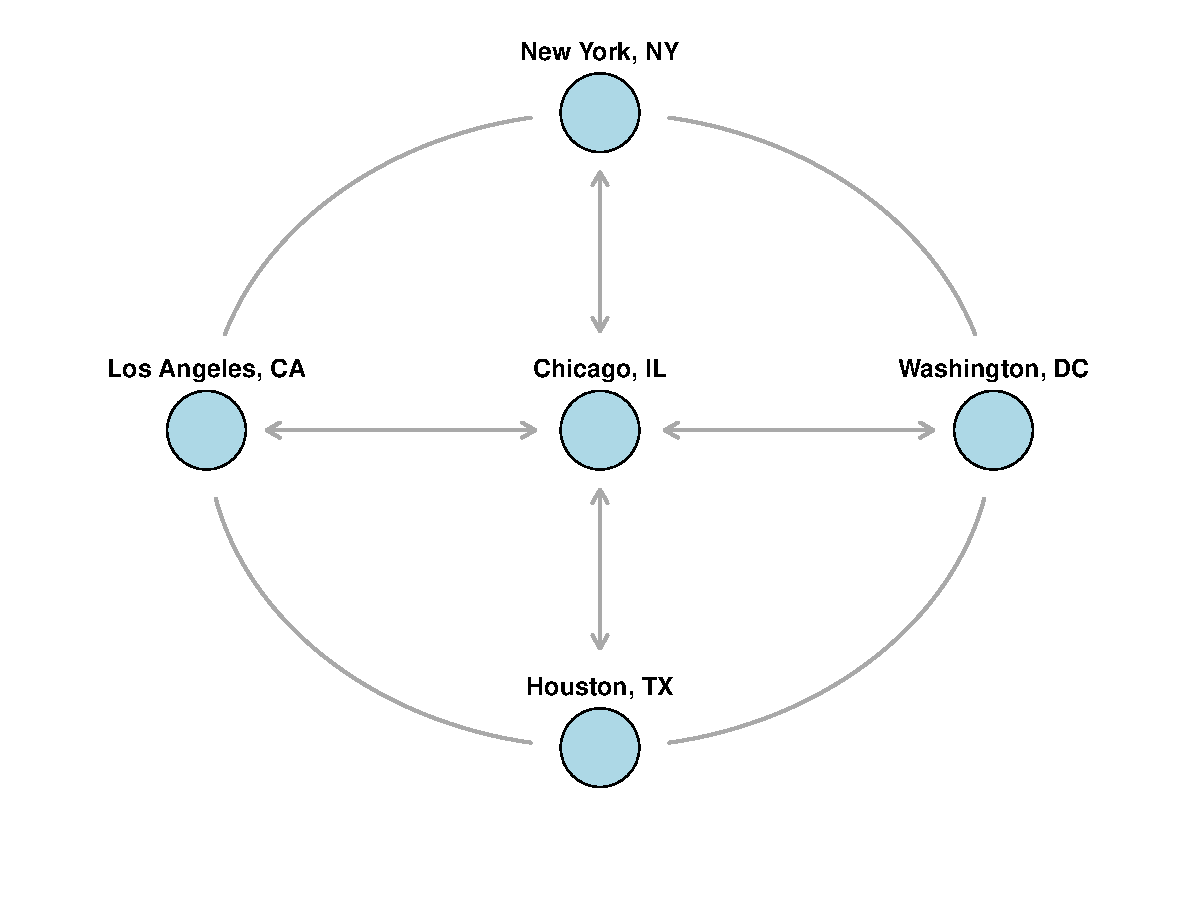
\includegraphics{figures/ModelFigure2.png}
\caption{}
\end{figure}

\end{frame}

\begin{frame}{Model design}

\begin{figure}
\centering
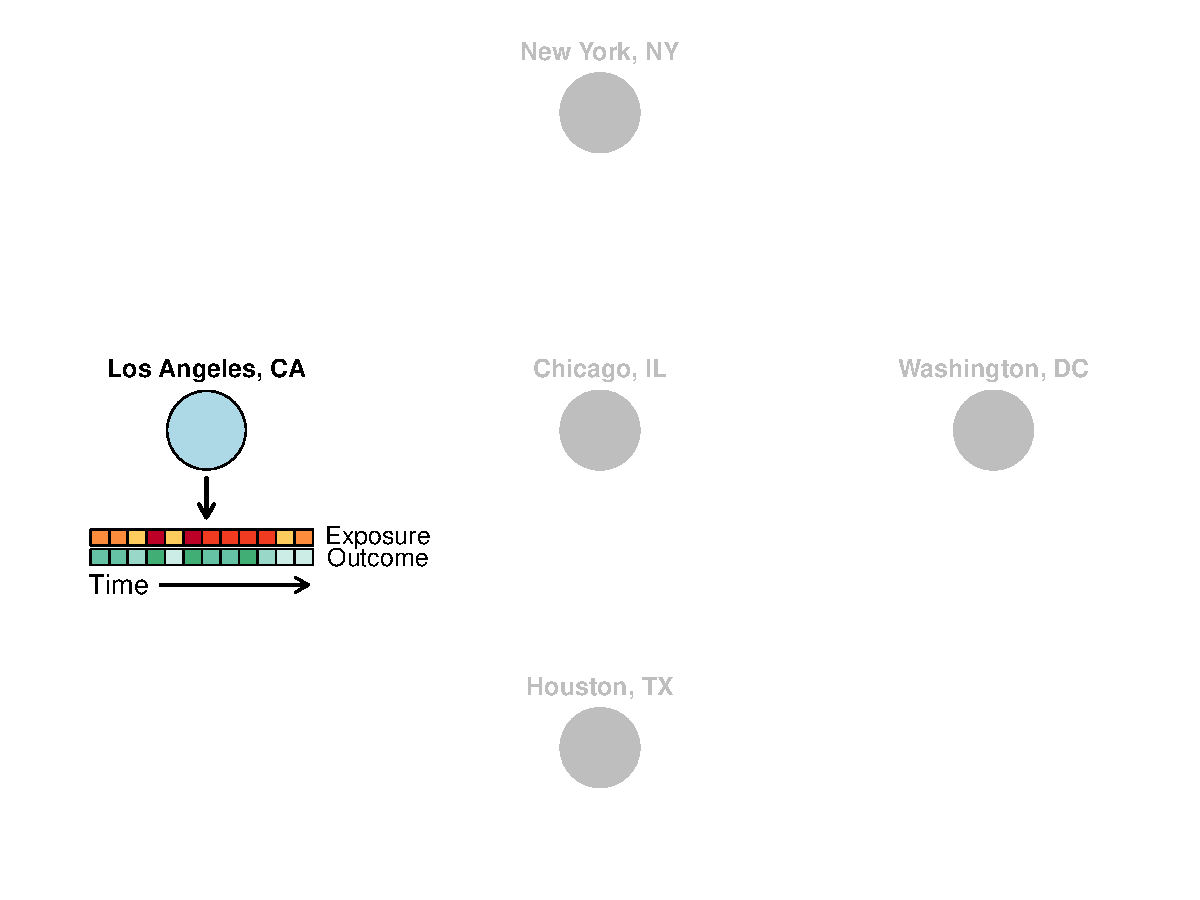
\includegraphics{figures/ModelFigure3.png}
\caption{}
\end{figure}

\end{frame}

\begin{frame}{Model design}

\begin{figure}
\centering
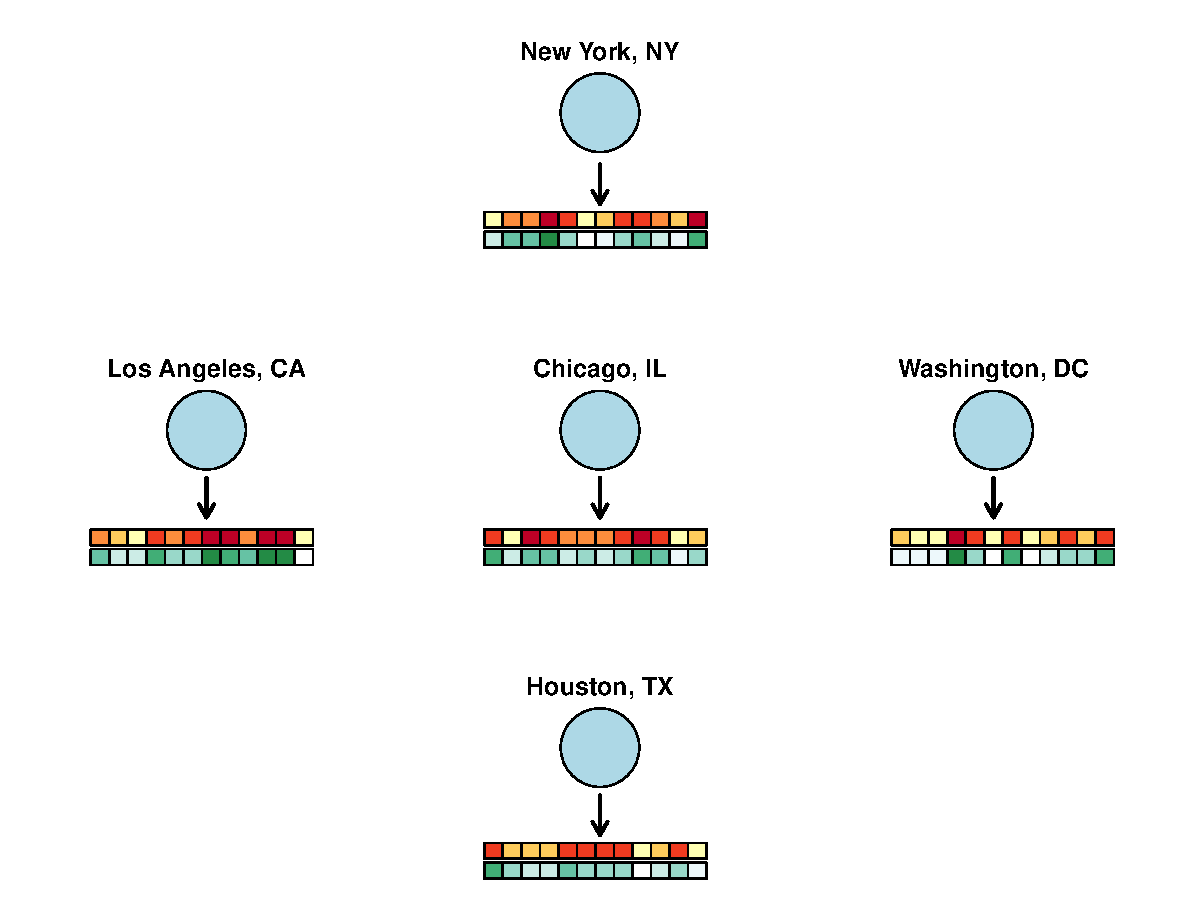
\includegraphics{figures/ModelFigure4.png}
\caption{}
\end{figure}

\end{frame}

\begin{frame}{Model design}

The model we fit is:

\[
Y(t) \sim Quasipoisson(\mu_t, \sigma^2)
\] \[
log(\mu_t) = \beta_{0} + \beta_{1}PM_{t} + f(t) + Z(t)
\]

\end{frame}

\begin{frame}{Confounders}

\includegraphics{figures/feb_13_2018/plot-unnamed-chunk-6-1.pdf}

\end{frame}

\begin{frame}{Confounders}

\includegraphics{figures/feb_13_2018/plot-unnamed-chunk-7-1.pdf}

\end{frame}

\begin{frame}{Confounders}

\begin{itemize}
\tightlist
\item
  Measured confounders

  \begin{itemize}
  \tightlist
  \item
    Temperature
  \item
    Dew point temperature
  \item
    Day of the week
  \end{itemize}
\item
  Unmeasured confounders

  \begin{itemize}
  \tightlist
  \item
    Long-term time trends

    \begin{itemize}
    \tightlist
    \item
      Changing population size
    \item
      Changing population demographics
    \end{itemize}
  \item
    Seasonal time trends

    \begin{itemize}
    \tightlist
    \item
      Respiratory infections
    \item
      Influenza
    \end{itemize}
  \end{itemize}
\end{itemize}

\end{frame}

\begin{frame}{Controlling for confounders}

Some cofounders you might want to fit using a more complex form. For
example, the relationship between temperature and mortality is often
non-linear, with the lowest risk at mild temperatures and increasing
risk as temperature gets colder or hotter.

\end{frame}

\begin{frame}{Splines}

\begin{figure}
\centering
\includegraphics{figures/Spline.png}
\caption{}
\end{figure}

\emph{Source: Wikipedia}

\end{frame}

\begin{frame}{Choosing degrees of freedom}

\begin{itemize}
\tightlist
\item
  Data-driven: Minimize a goodness-of-fit metric
\item
  \emph{A priori}: Use a reasonable value based on prior knowledge
\end{itemize}

\end{frame}

\begin{frame}{Convergence: ``GAM-gate''}

\begin{figure}
\centering
\includegraphics{figures/GAMgate.png}
\caption{}
\end{figure}

\end{frame}

\section{Implementation: Time series
studies}\label{implementation-time-series-studies}

\begin{frame}[fragile]{Overdispersed Poisson example}

For example, say we wanted to fit an overdispersed Poisson regression
for the \texttt{chic} data of whether cardiovascular mortality is
associated with particulate matter (note: in this simplified example,
I'm not controlling for many things we normally would, like season and
temperature).

\begin{Shaded}
\begin{Highlighting}[]
\NormalTok{mod_d <-}\StringTok{ }\KeywordTok{glm}\NormalTok{(cvd }\OperatorTok{~}\StringTok{ }\NormalTok{pm10, }\DataTypeTok{data =}\NormalTok{ chic,}
             \DataTypeTok{family =} \KeywordTok{quasipoisson}\NormalTok{())}
\KeywordTok{summary}\NormalTok{(mod_d)}\OperatorTok{$}\NormalTok{coef[ , }\KeywordTok{c}\NormalTok{(}\DecValTok{1}\NormalTok{, }\DecValTok{2}\NormalTok{, }\DecValTok{4}\NormalTok{)]}
\end{Highlighting}
\end{Shaded}

\begin{verbatim}
##                  Estimate   Std. Error  Pr(>|t|)
## (Intercept)  3.9327868499 0.0059351054 0.0000000
## pm10        -0.0001760049 0.0001530262 0.2501337
\end{verbatim}

\end{frame}

\begin{frame}{Overdispersed Poisson example}

Here, the model coefficient gives the \textbf{log relative risk} of
cardiovascular mortality associated with a unit increase in PM10
concentration.

\end{frame}

\begin{frame}[fragile]{Controlling for confounders}

We usually want to control for other confounders. For example, when we
look at the association between PM10 and cardiovascular mortality, we
probably want to control for things like day of the week, seasonal and
long-term mortality trends, and temperature.

We can control for these potential confounders by adding them in to the
right-hand side of the formula:

\begin{Shaded}
\begin{Highlighting}[]
\CommentTok{# Note: This is pseudocode}
\NormalTok{[health outcome] }\OperatorTok{~}\StringTok{ }\NormalTok{[exposure of interest] }\OperatorTok{+}\StringTok{ }
\StringTok{                   }\NormalTok{[confounder1] }\OperatorTok{+}\StringTok{ }\NormalTok{[confounder }\DecValTok{2}\NormalTok{] ...}
\end{Highlighting}
\end{Shaded}

\end{frame}

\begin{frame}[fragile]{Controlling for confounders}

For example, we usually want to control for day of the week as a factor.
To do that, first make sure that day of the week has the class
\texttt{factor}:

\begin{Shaded}
\begin{Highlighting}[]
\KeywordTok{class}\NormalTok{(chic}\OperatorTok{$}\NormalTok{dow)}
\end{Highlighting}
\end{Shaded}

\begin{verbatim}
## [1] "factor"
\end{verbatim}

\end{frame}

\begin{frame}[fragile]{Controlling for confounders}

If so, you can include it in your model:

\begin{Shaded}
\begin{Highlighting}[]
\NormalTok{mod_e <-}\StringTok{ }\KeywordTok{glm}\NormalTok{(cvd }\OperatorTok{~}\StringTok{ }\NormalTok{pm10 }\OperatorTok{+}\StringTok{ }\NormalTok{dow, }\DataTypeTok{data =}\NormalTok{ chic,}
             \DataTypeTok{family =} \KeywordTok{quasipoisson}\NormalTok{())}
\KeywordTok{summary}\NormalTok{(mod_e)}\OperatorTok{$}\NormalTok{coef[ , }\KeywordTok{c}\NormalTok{(}\DecValTok{1}\NormalTok{, }\DecValTok{2}\NormalTok{, }\DecValTok{4}\NormalTok{)]}
\end{Highlighting}
\end{Shaded}

\begin{verbatim}
##                  Estimate   Std. Error     Pr(>|t|)
## (Intercept)   3.914136910 0.0089931211 0.000000e+00
## pm10         -0.000211628 0.0001550096 1.722355e-01
## dowMonday     0.048178938 0.0111293675 1.528087e-05
## dowTuesday    0.030462708 0.0111124226 6.141692e-03
## dowWednesday  0.011251065 0.0111850000 3.145106e-01
## dowThursday   0.012227882 0.0111654287 2.735028e-01
## dowFriday     0.019722730 0.0111817715 7.782369e-02
## dowSaturday   0.016837469 0.0111119395 1.297719e-01
\end{verbatim}

\end{frame}

\begin{frame}[fragile]{Controlling for confounders}

You can use \texttt{ns()} from the \texttt{splines} package to fit
temperature using a spline. Here, I am fitting a spline with four
degrees of freedom:

\begin{Shaded}
\begin{Highlighting}[]
\KeywordTok{library}\NormalTok{(splines)}
\NormalTok{mod_e <-}\StringTok{ }\KeywordTok{glm}\NormalTok{(cvd }\OperatorTok{~}\StringTok{ }\NormalTok{pm10 }\OperatorTok{+}\StringTok{ }\NormalTok{dow }\OperatorTok{+}\StringTok{ }\KeywordTok{ns}\NormalTok{(temp, }\DecValTok{4}\NormalTok{),}
             \DataTypeTok{data =}\NormalTok{ chic,}
             \DataTypeTok{family =} \KeywordTok{quasipoisson}\NormalTok{())}
\KeywordTok{summary}\NormalTok{(mod_e)}\OperatorTok{$}\NormalTok{coef[}\KeywordTok{c}\NormalTok{(}\DecValTok{1}\OperatorTok{:}\DecValTok{2}\NormalTok{, }\DecValTok{9}\OperatorTok{:}\DecValTok{12}\NormalTok{), }\KeywordTok{c}\NormalTok{(}\DecValTok{1}\NormalTok{, }\DecValTok{2}\NormalTok{, }\DecValTok{4}\NormalTok{)]}
\end{Highlighting}
\end{Shaded}

\begin{verbatim}
##                   Estimate   Std. Error     Pr(>|t|)
## (Intercept)   4.0533073621 0.0357364704 0.000000e+00
## pm10          0.0008714696 0.0001579088 3.590381e-08
## ns(temp, 4)1 -0.1767349276 0.0318373157 2.988366e-08
## ns(temp, 4)2 -0.3278324170 0.0254813081 2.842988e-37
## ns(temp, 4)3 -0.1992809283 0.0743260391 7.361296e-03
## ns(temp, 4)4 -0.0279239953 0.0272149287 3.049171e-01
\end{verbatim}

\end{frame}

\begin{frame}[fragile]{Controlling for confounders}

Controlling for seasonal and long-term trends is similar. Often, we will
use a spline with around 7 degrees of freedom per year. To fit this,
first find out how many years are in your data:

\begin{Shaded}
\begin{Highlighting}[]
\KeywordTok{length}\NormalTok{(}\KeywordTok{unique}\NormalTok{(chic}\OperatorTok{$}\NormalTok{date)) }\OperatorTok{/}\StringTok{ }\DecValTok{365}
\end{Highlighting}
\end{Shaded}

\begin{verbatim}
## [1] 14.01096
\end{verbatim}

\end{frame}

\begin{frame}[fragile]{Controlling for confounders}

Then add a column for \texttt{time}:

\begin{Shaded}
\begin{Highlighting}[]
\NormalTok{chic}\OperatorTok{$}\NormalTok{time <-}\StringTok{ }\KeywordTok{scale}\NormalTok{(chic}\OperatorTok{$}\NormalTok{date, }\DataTypeTok{scale =} \OtherTok{FALSE}\NormalTok{,}
                   \DataTypeTok{center =} \OtherTok{TRUE}\NormalTok{)}
\NormalTok{chic}\OperatorTok{$}\NormalTok{time[}\DecValTok{1}\OperatorTok{:}\DecValTok{3}\NormalTok{]}
\end{Highlighting}
\end{Shaded}

\begin{verbatim}
## [1] -2556.5 -2555.5 -2554.5
\end{verbatim}

\begin{Shaded}
\begin{Highlighting}[]
\KeywordTok{summary}\NormalTok{(chic}\OperatorTok{$}\NormalTok{time)}
\end{Highlighting}
\end{Shaded}

\begin{verbatim}
##        V1       
##  Min.   :-2556  
##  1st Qu.:-1278  
##  Median :    0  
##  Mean   :    0  
##  3rd Qu.: 1278  
##  Max.   : 2556
\end{verbatim}

\end{frame}

\begin{frame}[fragile]{Controlling for confounders}

Now you can fit the model:

\begin{Shaded}
\begin{Highlighting}[]
\NormalTok{mod_e <-}\StringTok{ }\KeywordTok{glm}\NormalTok{(cvd }\OperatorTok{~}\StringTok{ }\NormalTok{pm10 }\OperatorTok{+}\StringTok{ }\NormalTok{dow }\OperatorTok{+}\StringTok{ }\KeywordTok{ns}\NormalTok{(temp, }\DecValTok{4}\NormalTok{) }\OperatorTok{+}
\StringTok{             }\KeywordTok{ns}\NormalTok{(time, }\DecValTok{7} \OperatorTok{*}\StringTok{ }\DecValTok{14}\NormalTok{),}
             \DataTypeTok{data =}\NormalTok{ chic,}
             \DataTypeTok{family =} \KeywordTok{quasipoisson}\NormalTok{())}
\KeywordTok{summary}\NormalTok{(mod_e)}\OperatorTok{$}\NormalTok{coef[}\KeywordTok{c}\NormalTok{(}\DecValTok{1}\OperatorTok{:}\DecValTok{2}\NormalTok{, }\DecValTok{13}\OperatorTok{:}\DecValTok{15}\NormalTok{), }\KeywordTok{c}\NormalTok{(}\DecValTok{1}\NormalTok{, }\DecValTok{2}\NormalTok{, }\DecValTok{4}\NormalTok{)]}
\end{Highlighting}
\end{Shaded}

\begin{verbatim}
##                       Estimate   Std. Error     Pr(>|t|)
## (Intercept)        4.162023561 0.0583344638 0.0000000000
## pm10               0.000202813 0.0001540345 0.1880118867
## ns(time, 7 * 14)1 -0.059709991 0.0583191728 0.3059589958
## ns(time, 7 * 14)2 -0.181691561 0.0770088168 0.0183466812
## ns(time, 7 * 14)3 -0.240738856 0.0700453542 0.0005934585
\end{verbatim}

\end{frame}

\begin{frame}[fragile]{Controlling for convergence problems}

One way to account for ``GAM-gate'' is to change the convergence default
threshold using the \texttt{control} option in \texttt{glm}:

\begin{Shaded}
\begin{Highlighting}[]
\NormalTok{mod_e <-}\StringTok{ }\KeywordTok{glm}\NormalTok{(cvd }\OperatorTok{~}\StringTok{ }\NormalTok{pm10 }\OperatorTok{+}\StringTok{ }\NormalTok{dow }\OperatorTok{+}\StringTok{ }\KeywordTok{ns}\NormalTok{(temp, }\DecValTok{4}\NormalTok{) }\OperatorTok{+}\StringTok{ }
\StringTok{                   }\KeywordTok{ns}\NormalTok{(time, }\DecValTok{7} \OperatorTok{*}\StringTok{ }\DecValTok{14}\NormalTok{),}
             \DataTypeTok{data =}\NormalTok{ chic,}
             \DataTypeTok{family =} \KeywordTok{quasipoisson}\NormalTok{(),}
             \DataTypeTok{control =} \KeywordTok{glm.control}\NormalTok{(}\DataTypeTok{epsilon=}\FloatTok{10E-8}\NormalTok{,}
                                 \DataTypeTok{maxit =} \DecValTok{10000}\NormalTok{))}
\end{Highlighting}
\end{Shaded}

Generally, it is good practice to include this when modeling air
pollution-health relationships.

\end{frame}

\begin{frame}[fragile]{Interpreting model coefficients}

You can pull the model coefficient you're interested in from the model
summary using this code:

\begin{Shaded}
\begin{Highlighting}[]
\NormalTok{pm_coef <-}\StringTok{ }\KeywordTok{summary}\NormalTok{(mod_e)}\OperatorTok{$}\NormalTok{coefficients[}\StringTok{"pm10"}\NormalTok{, ]}
\NormalTok{pm_coef}
\end{Highlighting}
\end{Shaded}

\begin{verbatim}
##     Estimate   Std. Error      t value     Pr(>|t|) 
## 0.0002028130 0.0001540345 1.3166725629 0.1880118867
\end{verbatim}

\end{frame}

\begin{frame}[fragile]{Interpreting model coefficients}

Remember that this model coefficient is the \textbf{log} relative risk,
since we fit a quasi-Poisson model. To get a relative risk estimate,
you'll need to take the exponent:

\begin{Shaded}
\begin{Highlighting}[]
\KeywordTok{exp}\NormalTok{(pm_coef[}\DecValTok{1}\NormalTok{])}
\end{Highlighting}
\end{Shaded}

\begin{verbatim}
## Estimate 
## 1.000203
\end{verbatim}

Therefore, there is a relative risk of 1.0002028 for each increase of 1
\(\mu{g}/m^3\) PM10.

\end{frame}

\begin{frame}[fragile]{Interpreting model coefficients}

Often, epidemiology studies will present relative risk for a 10-unit,
rather than 1-unit, increase in exposure (e.g., per 10 \(\mu{g}/m^3\)
PM10). To estimate this, you need to multiple the coefficient by 10
\emph{before} taking the exponential:

\begin{Shaded}
\begin{Highlighting}[]
\KeywordTok{exp}\NormalTok{(}\DecValTok{10} \OperatorTok{*}\StringTok{ }\NormalTok{pm_coef[}\DecValTok{1}\NormalTok{])}
\end{Highlighting}
\end{Shaded}

\begin{verbatim}
## Estimate 
##  1.00203
\end{verbatim}

Therefore, there is a relative risk of 1.0020302 for an increase of 10
\(\mu{g}/m^3\) PM10.

\end{frame}

\begin{frame}[fragile]{Interpreting model coefficients}

Sometimes, epidemiology studies will present results as \% increase in
mortality instead of relative risk. You can calculate this as:

\% increase = 100 * (RR - 1)

For our example model, you could calculate:

\begin{Shaded}
\begin{Highlighting}[]
\DecValTok{100} \OperatorTok{*}\StringTok{ }\NormalTok{(}\KeywordTok{exp}\NormalTok{(}\DecValTok{10} \OperatorTok{*}\StringTok{ }\NormalTok{pm_coef[}\DecValTok{1}\NormalTok{]) }\OperatorTok{-}\StringTok{ }\DecValTok{1}\NormalTok{)}
\end{Highlighting}
\end{Shaded}

\begin{verbatim}
##  Estimate 
## 0.2030188
\end{verbatim}

Therefore, there is a 0.203\% increase in mortality for an increase of
10 \(\mu{g}/m^3\) PM10.

\end{frame}

\section{Concept: Case-crossover
studies}\label{concept-case-crossover-studies}

\begin{frame}{Case-crossover models}

Case-crossover model designs are based on the idea of matched
case-control studies. For these, instead of comparing averages of
exposure for cases versus controls, you compare the average difference
across each matched set of case and control(s).

\includegraphics{figures/feb_13_2018/plot-unnamed-chunk-21-1.pdf}

\end{frame}

\begin{frame}{Types of case-crossover designs}

\begin{figure}
\centering
\includegraphics{figures/CaseCrossTypes.jpg}
\caption{}
\end{figure}

\emph{Source: Sorock et al. 2001, Injury Prevention}

\end{frame}

\begin{frame}{Strata for case-crossover}

\includegraphics{figures/feb_13_2018/plot-unnamed-chunk-22-1.pdf}

\end{frame}

\begin{frame}{Concept of case-crossover}

For each death in the dataset: Given that the death happened on one of
the days in its strata, what is the probability that it happened on the
day it did?

\[
Pr(Death | Stratum, Exposure)
\]

\end{frame}

\begin{frame}{Conditional logistic vs.~GLM}

\begin{figure}
\centering
\includegraphics{figures/ZegerLu.png}
\caption{}
\end{figure}

\end{frame}

\begin{frame}{Conditional logistic vs.~GLM}

\begin{quote}
``In this paper, we show that case-crossover using conditional logistic
regression is a special case of time series analysis when there is a
common exposure such as in air pollution studies. This equivalence
provides computational convenience for case-crossover analyses and a
better understanding of time series models.''
\end{quote}

\emph{Source: Lu and Zeger Biostatistics 2007}

\end{frame}

\begin{frame}{Conditional logistic vs.~GLM}

Case-crossover fit using a GLM:

\[
Y(t) \sim Quasipoisson(\mu_t, \sigma^2)
\] \[
log(\mu_t) = \beta_{0} + \beta_{1}PM_{t} + \beta_{2}Stratum_{t} + Z(t)
\]

\end{frame}

\begin{frame}{Conditional logistic vs.~GLM}

\begin{figure}
\centering
\includegraphics{figures/Armstrong1.png}
\caption{}
\end{figure}

\emph{Source: Armstrong et al. BMC Medical Research Methodology 2014}

\end{frame}

\begin{frame}{Conditional logistic vs.~GLM}

\begin{figure}
\centering
\includegraphics{figures/Armstrong2.png}
\caption{}
\end{figure}

\emph{Source: Armstrong et al. BMC Medical Research Methodology 2014}

\end{frame}

\section{Implementation: Case-crossover
studies}\label{implementation-case-crossover-studies}

\begin{frame}[fragile]{GLM method}

To code using a GLM, first you need to create a column with the stratum.
In R, you can use \texttt{format} with the date to do this easily, and
then convert the formatted date for a \texttt{factor} class:

\begin{Shaded}
\begin{Highlighting}[]
\NormalTok{chic}\OperatorTok{$}\NormalTok{casecross_stratum <-}\StringTok{ }\KeywordTok{format}\NormalTok{(chic}\OperatorTok{$}\NormalTok{date, }\StringTok{"%Y-%m-%a"}\NormalTok{)}
\NormalTok{chic}\OperatorTok{$}\NormalTok{casecross_stratum <-}\StringTok{ }\KeywordTok{factor}\NormalTok{(chic}\OperatorTok{$}\NormalTok{casecross_stratum)}
\KeywordTok{head}\NormalTok{(chic}\OperatorTok{$}\NormalTok{casecross_stratum, }\DecValTok{3}\NormalTok{)}
\end{Highlighting}
\end{Shaded}

\begin{verbatim}
## [1] 1987-01-Thu 1987-01-Fri 1987-01-Sat
## 1176 Levels: 1987-01-Fri 1987-01-Mon 1987-01-Sat 1987-01-Sun ... 2000-12-Wed
\end{verbatim}

\end{frame}

\begin{frame}[fragile]{Case-crossover}

Now you can include this factor in your model (note: this takes the
place of model control for time trends and day of week in a typical time
series model):

\begin{Shaded}
\begin{Highlighting}[]
\NormalTok{mod_f <-}\StringTok{ }\KeywordTok{glm}\NormalTok{(cvd }\OperatorTok{~}\StringTok{ }\NormalTok{pm10 }\OperatorTok{+}\StringTok{ }\KeywordTok{ns}\NormalTok{(temp, }\DecValTok{4}\NormalTok{) }\OperatorTok{+}\StringTok{ }\NormalTok{casecross_stratum,}
             \DataTypeTok{data =}\NormalTok{ chic,}
             \DataTypeTok{family =} \KeywordTok{quasipoisson}\NormalTok{())}
\KeywordTok{summary}\NormalTok{(mod_f)}\OperatorTok{$}\NormalTok{coef[}\KeywordTok{c}\NormalTok{(}\DecValTok{1}\OperatorTok{:}\DecValTok{2}\NormalTok{, }\DecValTok{7}\OperatorTok{:}\DecValTok{10}\NormalTok{), }\KeywordTok{c}\NormalTok{(}\DecValTok{1}\NormalTok{, }\DecValTok{2}\NormalTok{)]}
\end{Highlighting}
\end{Shaded}

\begin{verbatim}
##                                  Estimate   Std. Error
## (Intercept)                  4.0482946294 0.0855215089
## pm10                         0.0001909843 0.0001680322
## casecross_stratum1987-01-Mon 0.1907876393 0.1137590495
## casecross_stratum1987-01-Sat 0.0855529446 0.1168756412
## casecross_stratum1987-01-Sun 0.3300835895 0.1099033832
## casecross_stratum1987-01-Thu 0.0462517003 0.1043859066
\end{verbatim}

\end{frame}

\begin{frame}[fragile]{Case-crossover}

You can interpret the coefficients now in the same way as with the time
series model:

\begin{Shaded}
\begin{Highlighting}[]
\NormalTok{pm_coef <-}\StringTok{ }\KeywordTok{summary}\NormalTok{(mod_f)}\OperatorTok{$}\NormalTok{coefficients[}\StringTok{"pm10"}\NormalTok{, ]}
\DecValTok{100} \OperatorTok{*}\StringTok{ }\NormalTok{(}\KeywordTok{exp}\NormalTok{(}\DecValTok{10} \OperatorTok{*}\StringTok{ }\NormalTok{pm_coef[}\DecValTok{1}\NormalTok{]) }\OperatorTok{-}\StringTok{ }\DecValTok{1}\NormalTok{)}
\end{Highlighting}
\end{Shaded}

\begin{verbatim}
##  Estimate 
## 0.1911668
\end{verbatim}

Therefore, for this model, there is a 0.191\% increase in mortality for
an increase of 10 \(\mu{g}/m^3\) PM10.

\end{frame}

\begin{frame}[fragile]{Case-crossover}

There are also other methods for fitting case-crossover models:

\begin{itemize}
\tightlist
\item
  Armstrong et al. (Conditional Poisson models: a flexible alternative
  to conditional logistic case cross-over analysis) suggest using a
  conditional Poisson regression model (\texttt{gnm()}) to speed up
  computational time.
\item
  The \texttt{casecross} function in the \texttt{season} package by
  Adrian Barnett uses 28-day strata (rather than by month) and a Cox
  proportional hazards regression model to fit the model.
\end{itemize}

If you are using this method for a paper, it is worthwhile testing the
different methods to see if you get similar results.

\end{frame}

\begin{frame}[fragile]{Case-crossover}

Using a conditional Poisson model:

\begin{Shaded}
\begin{Highlighting}[]
\KeywordTok{library}\NormalTok{(gnm)}
\NormalTok{mod_g <-}\StringTok{ }\KeywordTok{gnm}\NormalTok{(cvd }\OperatorTok{~}\StringTok{ }\NormalTok{pm10 }\OperatorTok{+}\StringTok{ }\KeywordTok{ns}\NormalTok{(temp, }\DecValTok{4}\NormalTok{),}
             \DataTypeTok{eliminate =}\NormalTok{ casecross_stratum,}
             \DataTypeTok{data =}\NormalTok{ chic,}
             \DataTypeTok{family =} \KeywordTok{quasipoisson}\NormalTok{())}
\NormalTok{pm_coef <-}\StringTok{ }\KeywordTok{summary}\NormalTok{(mod_g)}\OperatorTok{$}\NormalTok{coefficients[}\StringTok{"pm10"}\NormalTok{, ]}
\DecValTok{100} \OperatorTok{*}\StringTok{ }\NormalTok{(}\KeywordTok{exp}\NormalTok{(}\DecValTok{10} \OperatorTok{*}\StringTok{ }\NormalTok{pm_coef[}\DecValTok{1}\NormalTok{]) }\OperatorTok{-}\StringTok{ }\DecValTok{1}\NormalTok{)}
\end{Highlighting}
\end{Shaded}

\begin{verbatim}
##  Estimate 
## 0.1911668
\end{verbatim}

\end{frame}

\begin{frame}[fragile]{Case-crossover}

Using a Cox proportional hazards regression model:

\begin{Shaded}
\begin{Highlighting}[]
\KeywordTok{library}\NormalTok{(season)}
\NormalTok{mod_h <-}\StringTok{ }\KeywordTok{casecross}\NormalTok{(cvd }\OperatorTok{~}\StringTok{ }\NormalTok{pm10 }\OperatorTok{+}\StringTok{ }\NormalTok{temp,}
                   \DataTypeTok{matchdow =} \OtherTok{TRUE}\NormalTok{,}
                   \DataTypeTok{data =}\NormalTok{ chic)}
\end{Highlighting}
\end{Shaded}

\begin{verbatim}
## Note, irregularly spaced data...
## ...check your data for missing days
\end{verbatim}

\begin{Shaded}
\begin{Highlighting}[]
\NormalTok{pm_coef <-}\StringTok{ }\NormalTok{mod_h}\OperatorTok{$}\NormalTok{c.model}\OperatorTok{$}\NormalTok{coefficients[}\DecValTok{1}\NormalTok{]}
\DecValTok{100} \OperatorTok{*}\StringTok{ }\NormalTok{(}\KeywordTok{exp}\NormalTok{(}\DecValTok{10} \OperatorTok{*}\StringTok{ }\NormalTok{pm_coef[}\DecValTok{1}\NormalTok{]) }\OperatorTok{-}\StringTok{ }\DecValTok{1}\NormalTok{)}
\end{Highlighting}
\end{Shaded}

\begin{verbatim}
##      pm10 
## 0.4320228
\end{verbatim}

\end{frame}

\section{Multi-city studies}\label{multi-city-studies}

\begin{frame}{Samet editorial}

\begin{figure}
\centering
\includegraphics{figures/Samet2002.png}
\caption{}
\end{figure}

\end{frame}

\begin{frame}{NMMAPS}

\begin{figure}
\centering
\includegraphics{figures/NMMAPS.png}
\caption{}
\end{figure}

\emph{Source: www.ihapss.jhsph.edu}

\end{frame}

\begin{frame}{NMMAPS package}

\begin{figure}
\centering
\includegraphics{figures/NMMAPSPackageStructure.pdf}
\caption{}
\end{figure}

\end{frame}

\begin{frame}{Impact of NMMAPS}

Research impacts of NMMAPS package

\begin{itemize}
\tightlist
\item
  As of November 2011, 67 publications had been published using this
  data, with 1,781 citations to these papers
\item
  Research using NMMAPS has been used by the US EPA in creating
  regulatory impact statements for air pollution (particulates and
  ozone)
\item
  ``Thanks to NMMAPS, there is probably no other country in the world
  with a greater understanding of the health effects of air pollution
  and heat waves in its population.''"
\end{itemize}

\emph{Source: Barnett, Huang, and Turner, ``Benefits of Publicly
Available Data'', Epidemiology 2012}

\end{frame}

\end{document}